\mysubsection{Sarah Häfele}{Impressionen}

\subsubsection{Impressionen Tag der Medien}
Zum Abschluss noch einige Fotos vom Aufbau und vom Tag der Medien. Im Anhang dazu finden sich die technischen Skizzen, die, teilweise veraltet, die Testaufbauten dokumentieren und der Projektgruppe als Planungshilfe dienten.

\begin{figure}[htbp]
	\centering
		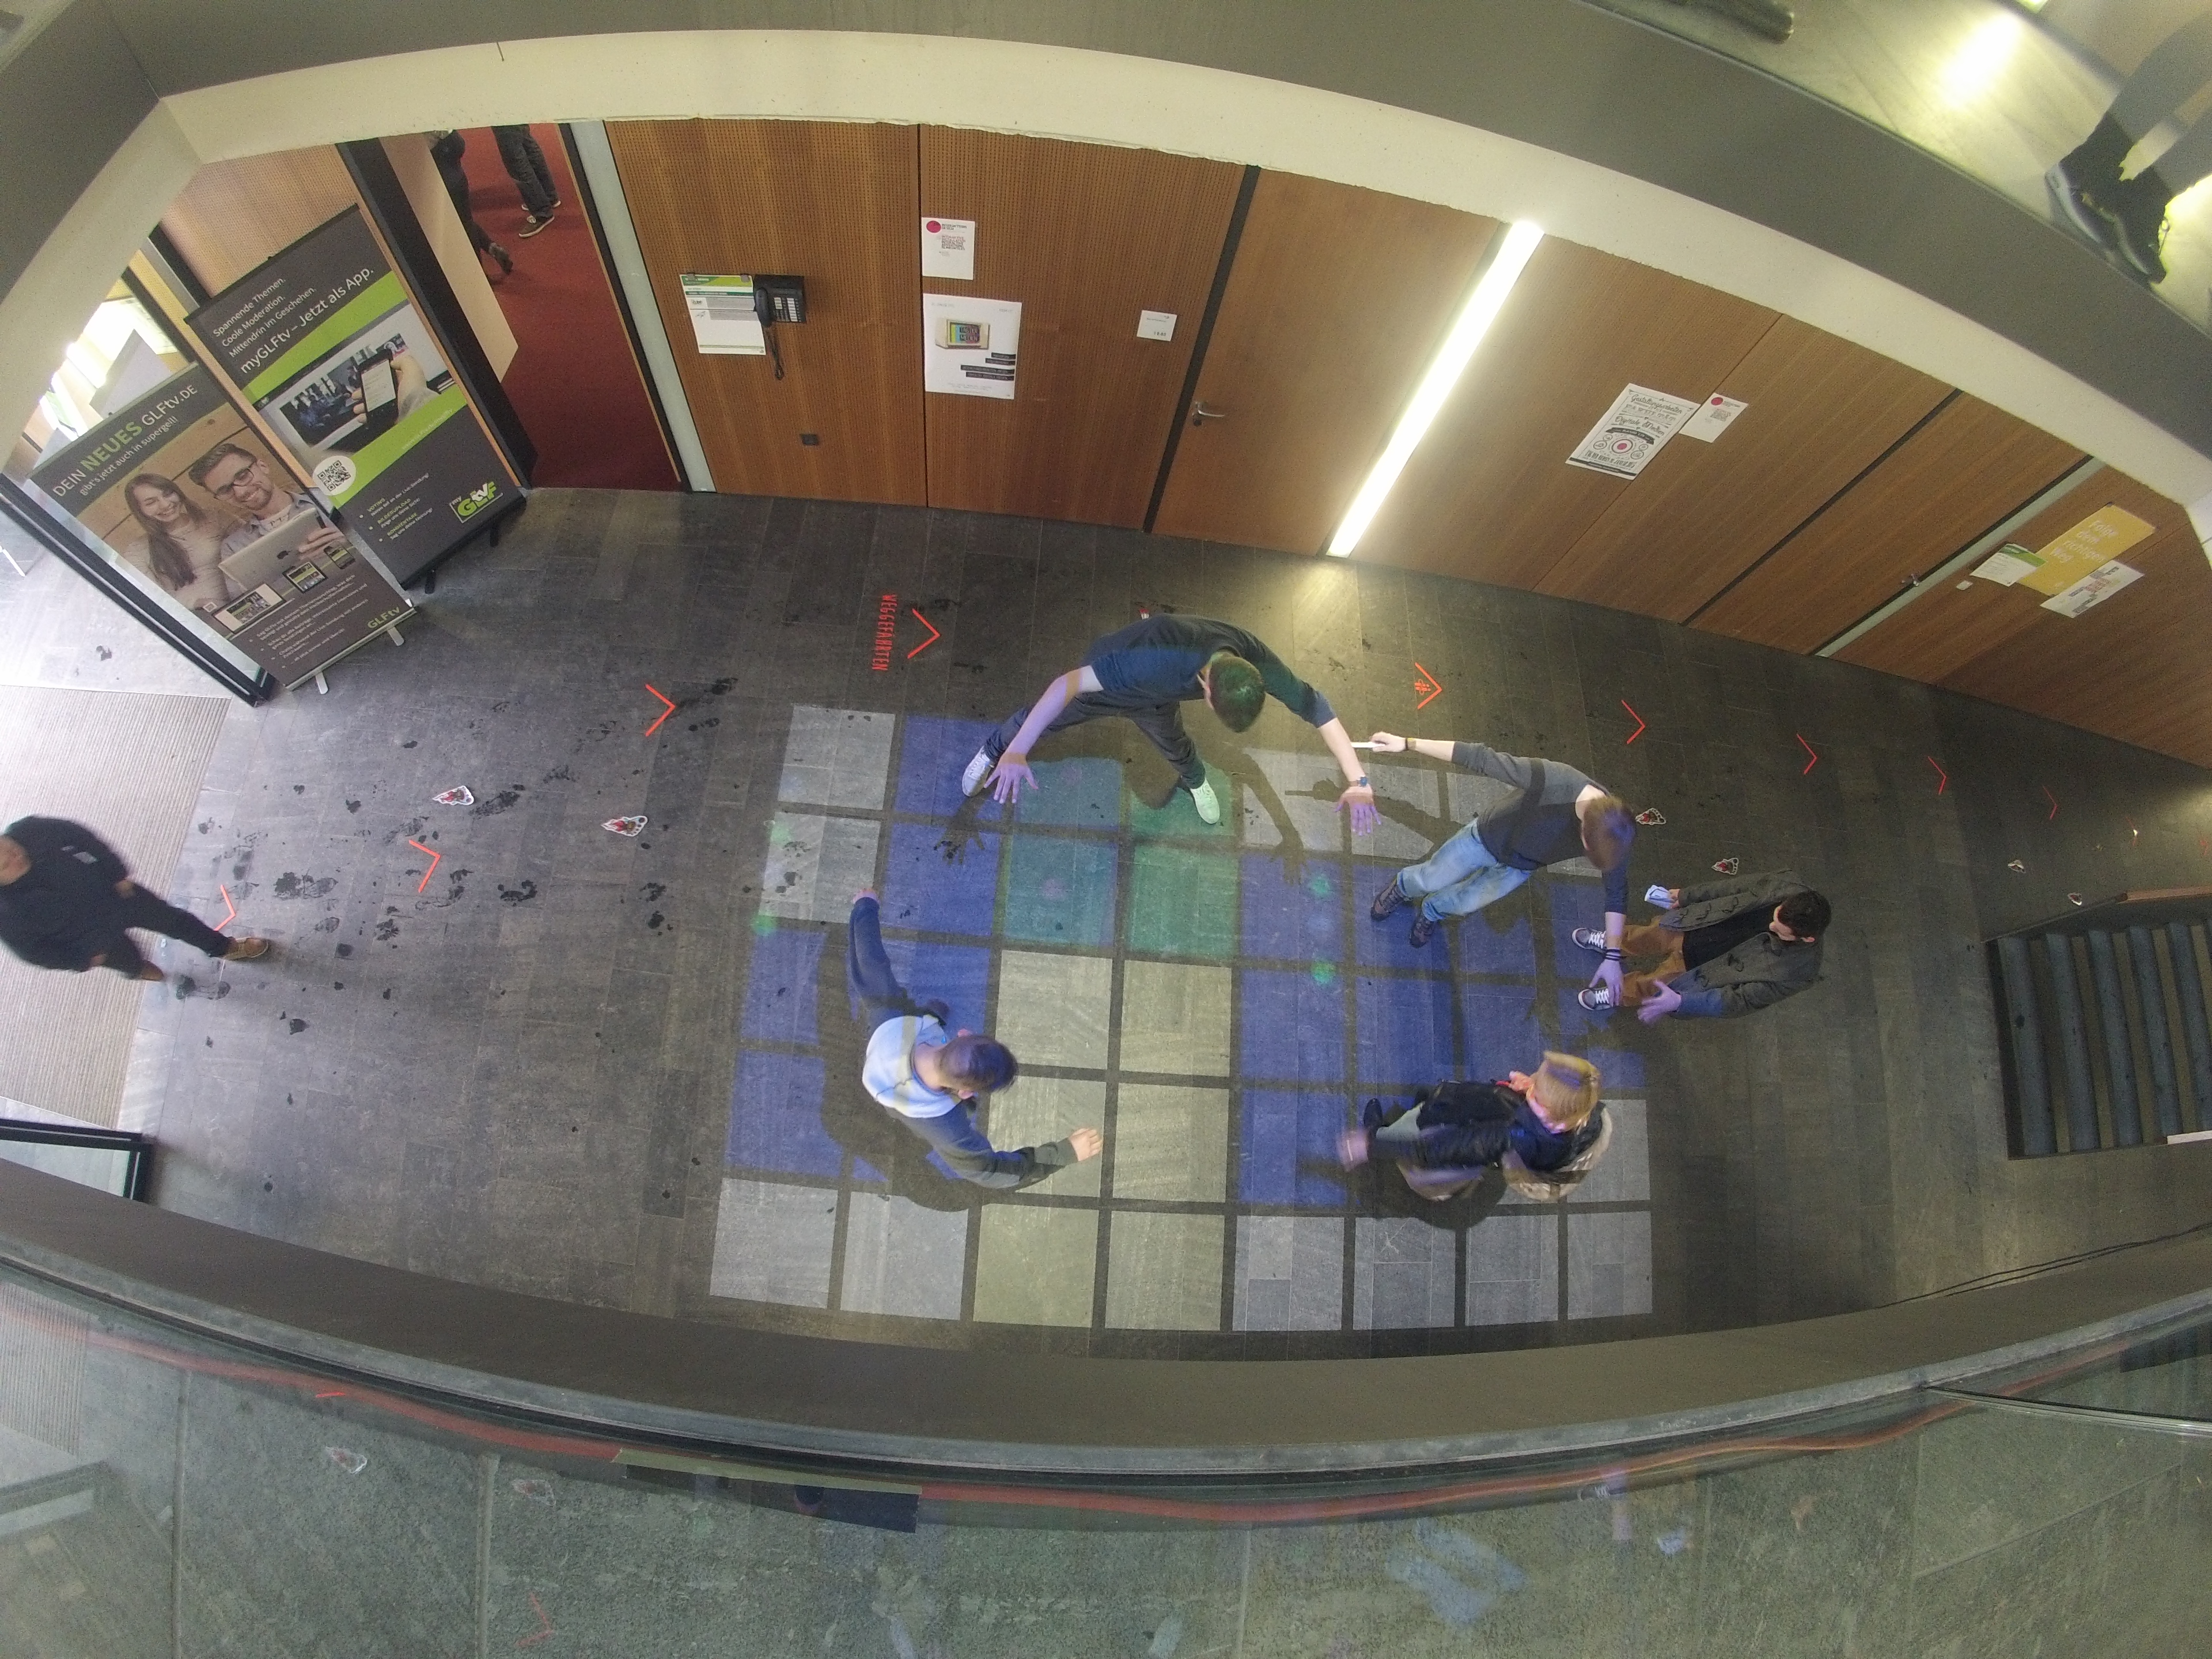
\includegraphics[width=0.9\textwidth]{images/TdM1.jpg}
	\caption{Installation von oben}
	\label{fig:TdM1}
\end{figure}

\begin{figure}[htbp]
	\centering
		\includegraphics[width=0.9\textwidth]{images/TdM2.jpg}
	\caption{Erdgeschoss \textit{(Foto: Ramazan Gündogdu)}}
	\label{fig:TdM2}
\end{figure}

\begin{figure}[htbp]
	\centering
		\includegraphics[width=0.9\textwidth]{images/TdM3.jpg}
	\caption{Traversenkonstruktion \textit{(Foto: Ramazan Gündogdu)}}
	\label{fig:TdM3}
\end{figure}

\begin{figure}[htbp]
	\centering
		\includegraphics[width=0.9\textwidth]{images/TdM4.jpg}
	\caption{Erster Stock Kontrollprogramm \textit{(Foto: Ramazan Gündogdu)}}
	\label{fig:TdM4}
\end{figure}

\begin{figure}[htbp]
	\centering
		\includegraphics[width=0.9\textwidth]{images/TdM5.jpg}
	\caption{Installation im Einsatz \textit{(Foto: GLF TV)}}
	\label{fig:TdM5}
\end{figure}
\clearpage

\subsubsection{Impressionen Erste Tests}
Die Installation wurde schon Wochen vor dem Tag der Medien in verschiedenen Varianten aufgebaut und auch an anderen Orten, wie in der Aula, getestet.

\begin{figure}[htbp]
	\centering
		\includegraphics[width=0.88\textwidth]{images/Test1.png}
	\caption{Tests mit zwei Beamern in der Aula}
	\label{fig:Test1}
\end{figure}

\begin{figure}[htbp]
	\centering
		\includegraphics[width=0.88\textwidth]{images/Test2.png}
	\caption{Tests mit der Kinect in der Aula}
	\label{fig:Test2}
\end{figure}

\begin{figure}[htbp]
	\centering
		\includegraphics[width=0.88\textwidth]{images/Test3.png}
	\caption{Tests mit der Kinect in der Aula}
	\label{fig:Test3}
\end{figure}

\begin{figure}[htbp]
	\centering
		\includegraphics[width=0.88\textwidth]{images/Test4.jpg}
	\caption{Erste Traversentests im I-Bau}
	\label{fig:Test4}
\end{figure}
\clearpage

\subsubsection{Technische Zeichnungen}
Die folgenden Seiten enthalten unter anderem die handgezeichneten technischen Zeichnungen und Bemaßungen, die während den Tests gemacht wurden.

\begin{figure}[htbp]
	\centering
		\includegraphics[width=0.9\textwidth]{images/TZ1.png}
	\caption{Erste Feldbemaßung}
	\label{fig:TZ1}
\end{figure}

\begin{figure}[htbp]
	\centering
		\includegraphics[width=0.9\textwidth]{images/TZ2.png}
	\caption{Ältere Beamer und Kinect Bemaßung}
	\label{fig:TZ2}
\end{figure}

\includepdf[pages=1-6]{images/TechnZeichnungen.pdf}